\documentclass[en,t]{sdqbeamer}
%\documentclass[c]{sdqbeamer}

\usepackage{listings}
\usepackage{graphicx}
\usepackage{tabularx}
\usepackage{multirow}
\usepackage{multicol}
\usepackage{tabulary}
\usepackage{colortbl}
\usepackage{tikzsymbols}
\usepackage{tikz}
\usepackage{booktabs}
\usetikzlibrary{positioning,fit,shapes}
\usepackage[lined,linesnumbered,ruled,noend]{algorithm2e}
\usepackage{bm}
\usepackage{forloop}

\hypersetup{
	colorlinks=true,
	urlcolor=kit-orange
}

% set sdqbeamer options
\titleimage{blender-render}
\groupname{Algorithm Engineering}
\grouplogo{ae}
%\selectlanguage{english}


\usepackage[backend=biber,style=numeric-comp,sorting=none]{biblatex}
\addbibresource{references.bib}

% define title etc.pp.
\title[SAT Solving]{Practical SAT Solving}
\subtitle{Lecture 14: SMT Solving}
\author{{Markus Iser}, \underline{Dominik Schreiber}, Tom\'a\v{s} Balyo}
\date{July 22, 2024}

% Existing KIT colors: kit-green, kit-blue, kit-red, kit-gray, kit-orange, kit-lightgreen, kit-brown, kit-purple, kit-cyan
% configure appearance
\setbeamercolor{block title}{bg=kit-blue}
\setbeamercolor{block body}{bg=kit-blue!10}
\setbeamercolor{block title example}{bg=kit-orange}
\setbeamercolor{block body example}{bg=kit-orange!10}
\setbeamertemplate{itemize item}{\color{kit-gray}\textbullet}
\setbeamertemplate{itemize subitem}{\color{kit-gray}\textbullet}
\setbeamercolor{item projected}{bg=kit-gray, fg=kit-gray}
\renewcommand{\insertnavigation}[1]{} % remove navigation bar

% define commands
\definecolor{myblue}{HTML}{0D3B66}
\definecolor{myred}{HTML}{6E0E0A}
\definecolor{mypink}{HTML}{F7B2B7}

\newcommand{\vars}[1]{\textsf{vars} (#1)}
\newcommand{\lits}[1]{\textsf{lits} (#1)}
\newcommand{\clss}[1]{\textsf{clss} (#1)}

\newcommand{\highl}[1]{\textcolor{myblue}{#1}}
\newcommand{\highlo}[1]{\textcolor{myred}{#1}}
\newcommand{\highlow}[1]{\textcolor{mypink}{#1}}

% Extra column types for tabularx
\newcolumntype{C}{>{\centering\arraybackslash}X}
\newcolumntype{L}{>{\raggedright\arraybackslash}X}
\newcolumntype{R}{>{\raggedleft\arraybackslash}X}

\newcommand{\setcolsep}[1]{\setlength{\tabcolsep}{#1}}
\newcommand{\setrowsep}[1]{\renewcommand{\arraystretch}{#1}}

% Definitions for the Tseitin transformation
\newcommand{\true}{\ensuremath{\mathit{True}}}
\newcommand{\false}{\ensuremath{\mathit{False}}}
\newcommand{\allvars}{\ensuremath{\mathcal{V}}}
\newcommand{\tseitin}[1]{\ensuremath{\mathcal{T}(#1)}}
\newcommand{\tseitinRec}[2]{\ensuremath{\mathcal{T}^{#2}(#1)}}
\newcommand{\tseitinSym}[1]{\ensuremath{\mathcal{T}_\mathsf{lit}(#1)}}
\newcommand{\tseitinDef}[2]{\ensuremath{\mathcal{T}_\mathsf{def}^{#2}(#1)}}
\newcommand{\hcancel}[2][black]{\setbox0=\hbox{$#2$}\rlap{\raisebox{.45\ht0}{\textcolor{#1}{\rule{\wd0}{1pt}}}}#2} 
\newcommand{\sateq}{\mathrel{\overset{\makebox[0pt]{\mbox{\normalfont\tiny\sffamily SAT}}}{=}}}

\newcommand{\enc}{\ensuremath{\mathcal{E}}} % encoding

% exercise commands
\newcommand{\exhead}[3]{
\hrule~\\[1ex]\noindent
{\bf Practical SAT Solving} (ST 2024) \hfill \fbox{Assignment #1} \\[1ex]
Markus Iser, Dominik Schreiber, Tom\'a\v{s} Balyo\\[1ex]
Algorithm Engineering (KIT) \hfill #2 -- #3\\
\hrule
\thispagestyle{empty}
}


\renewcommand{\highl}[1]{\textcolor{kit-blue}{#1}}
\renewcommand{\highlo}[1]{\textcolor{kit-orange}{#1}}
\newcommand{\unimp}[1]{\textcolor{gray}{#1}}

% Redefine `\rowcolor` to allow a beamer overlay specifier
% New syntax: \rewcolor<overlay>[color model]{color}[left overhang][right overhang]
\makeatletter
% Open `\noalign` and check for overlay specification:
\def\rowcolor{\noalign{\ifnum0=`}\fi\bmr@rowcolor}
\newcommand<>{\bmr@rowcolor}{%
    \alt#1%
        {\global\let\CT@do@color\CT@@do@color\@ifnextchar[\CT@rowa\CT@rowb}% Rest of original `\rowcolor`
        {\ifnum0=`{\fi}\@gooble@rowcolor}% End `\noalign` and gobble all arguments of `\rowcolor`.
}
% Gobble all normal arguments of `\rowcolor`:
\newcommand{\@gooble@rowcolor}[2][]{\@gooble@rowcolor@}
\newcommand{\@gooble@rowcolor@}[1][]{\@gooble@rowcolor@@}
\newcommand{\@gooble@rowcolor@@}[1][]{\ignorespaces}
\makeatother

% Redefine '\cellcolor' for beamer overlay use
\renewcommand<>\cellcolor[1]{\only#2{\beameroriginal\cellcolor{#1}}}

\begin{document}

\begin{frame}
	\thispagestyle{empty}
	\titlepage
\end{frame}

% \begin{minipage}[c][8cm][t]{0.65\textwidth}

\begin{frame}{Roadmap}

	\vspace*{-3mm}
	\begin{itemize}
		\item SMT: Motivation and definition
		\item Some example theories
		\item Formal framework and decidability
		\item SMT solving
		\begin{itemize}
			\item Lazy approach: DPLL($T$)
			\item Eager approach: The case of Bit Vectors
		\end{itemize}
		\item (Brief) pragmatics of SMT
	\end{itemize}

	\vspace*{4mm}

	\small
	\textbf{Note:} This lecture is mostly based on the following slide sets:\\

	\vspace*{2mm}
	\url{https://github.com/biotomas/sat-lecture-kit/blob/main/slides/l10.tex}\\
	\hfill\unimp{(motivation, example theories, decidability, DPLL(T) example, bit vectors)}
	
	\vspace*{2mm}
	\url{https://resources.mpi-inf.mpg.de/departments/rg1/conferences/vtsa08/slides/barret2_smt.pdf}\\
	\hfill\unimp{(formal definitions)}
	
	\vspace*{2mm}
	\url{https://alexeyignatiev.github.io/ssa-school-2019/slides/ao-satsmtar19-slides.pdf}\\
	\hfill\unimp{(lazy vs.\ eager, DPLL(T) techniques \& properties)}
\end{frame}

\begin{frame}{SMT: Motivation}
	\textbf{Propositional logic:} \highlo{very low-level} for many practical problems
	\begin{itemize}
		\item Linear (integer or real) \highl{arithmetic}:
		\[ x+y < 5 \wedge (2x-y > 4 \vee x+y > 7) \]
		\item \highl{Non-linear} arithmetic:
		\[ x^2 + y^2 = 4 \wedge x-y = 3 \]
		\item Arithmetic \highl{as actually done by a computer}:
		\[ 4294967295 + 1 = 0 \]
	\end{itemize}
	Natural point of extension: \textbf{First Order Logic} with suitable \highl{interpretation} / \highl{semantics}
\end{frame}

\begin{frame}{What is SMT?}
	\begin{block}{Satisfiability Modulo Theories (SMT)}
		Decide the satisfiability of a \highl{First Order Logic (FOL) formula} with respect to a certain \highl{background theory}.
	\end{block}
	\begin{itemize}
		\item \textbf{Syntax:} in most cases, \highl{quantifier-free, ground} fragment of FOL
		\begin{itemize}
			\item Set of atomic \highl{constants} \hfill \unimp{e.g., 0, 1, \texttt{null}}
			\item Set of $k$-ary \highl{functions} $f(x_1, \ldots, x_k)$ ($k \geq 1$) \hfill \unimp{e.g., +, $\times$, \texttt{read}, \texttt{write}}\\
			-- each $x_i$ is a \highl{term}, i.e., either a constant or some $k'$-ary function
			\vspace*{1mm}
			\item Set of $k$-ary \highl{propositions} $P(x_1, \ldots, x_k)$  \hfill \unimp{e.g., $=$, $<$}\\
			-- $k=0$: \highl{Atom} as in propositional logic\\
			-- each $x_i$ is a term
			\vspace*{1mm}
			\item Formula: Boolean expression featuring the above propositions as its ``variables''
		\end{itemize}
		\item \textbf{Semantics:} depends on chosen \highl{background theory}
		\begin{itemize}
			\item Many theories feature \highl{equality}, i.e., a special \highl{proposition} $P_=(x,y) \Leftrightarrow x=y$
			\item Each theory adds some set of \highl{axioms} that must hold
		\end{itemize}
	\end{itemize}
\end{frame}

\begin{frame}{Theory: Equality with Uninterpreted Functions (EUF)}
	\begin{itemize}
		\item Equality proposition ``$=$'' comes with some \highl{implicit axioms}:\\
		1. \highl{Reflexivity}: $\forall x:\ x=x$\\
		2. \highl{Symmetry}: $\forall x \, \forall y:\ x=y \rightarrow y=x$\\
		3. \highl{Transitivity}: $\forall x \, \forall y \, \forall z:\ x=y \wedge y=z \rightarrow x=z$\\
		4. \highl{Congruence}: $\forall k \, \forall f(x_1,\ldots,x_k) \, \forall x_1, \ldots, x_k \, \forall y_1, \ldots, y_k:\ $\\
		\phantom{4. \highl{Congruence}:} $\bigwedge_{i=1}^k x_i = y_i \rightarrow f(x_1,\ldots,x_k) = f(y_1,\ldots,y_k)$
		\item Functions are left \highl{uninterpreted} and thus carry \highl{no inherent meaning} apart from syntactical footprint
		\item Examples:\\
		\hspace*{1cm}$(z \neq x) \wedge (z \neq y)$ \hfill \highl{Satisfiable} for $\geq 3$ objects\\
		\hspace*{1cm}$h(a, g(f(b),f(c))) = d \wedge h(b,g(f(a),f(c))) \neq d \wedge a=b$ \hfill \highlo{Unsatisfiable}
		\item Useful to \highl{abstract away} non-supported constructions / operations
		\item Also called \highl{Theory of Equality}
	\end{itemize}
\end{frame}

\begin{frame}{Theory: Peano Arithmetic}
	\textbf{Arithmetic over natural numbers with addition and multiplication}
	\begin{itemize}
		\item Constants: $0, 1$\ \ \ \ $\cdot$\ \ \ \ Functions: $+, \times$\ \ \ \ $\cdot$\ \ \ \ Predicates: $=$
		\item Axioms:\\
		1. EUF axioms\\
		2. \highl{Null}: $\forall x:\ x+1 \neq 0$\\
		3. \highl{Successor}: $\forall x, y:\ x+1 = y+1 \rightarrow x = y$\\
		4. \highl{Induction}: $P(0) \wedge (\forall x:\ P(x) \rightarrow P(x+1)) \rightarrow (\forall x:\ P(x))$\\
		5. \highl{Plus Zero}: $\forall x:\ x+0=x$\\
		6. \highl{Plus successor}: $\forall x, y:\ x+(y+1) = (x+y)+1$\\
		7. \highl{Times Zero}: $\forall x:\ x \times 0 = 0$\\
		8. \highl{Times successor}: $\forall x,y:\ x \times (y+1) = (x \times y) + x$\\
	\end{itemize}
\end{frame}

\begin{frame}{Theory: Presburger Arithmetic}
	\textbf{Arithmetic over natural numbers with addition only}
	\begin{itemize}
		\item Constants: $0, 1$\ \ \ \ $\cdot$\ \ \ \ Functions: $+$\ \ \ \ $\cdot$\ \ \ \ Predicates: $=$
		\item Axioms:\\
		1. EUF axioms\\
		2. \highl{Null}: $\forall x:\ x+1 \neq 0$\\
		3. \highl{Successor}: $\forall x, y:\ x+1 = y+1 \rightarrow x = y$\\
		4. \highl{Induction}: $P(0) \wedge (\forall x:\ P(x) \rightarrow P(x+1)) \rightarrow (\forall x:\ P(x))$\\
		5. \highl{Plus Zero}: $\forall x:\ x+0=x$\\
		6. \highl{Plus successor}: $\forall x, y:\ x+(y+1) = (x+y)+1$\\
	\end{itemize}
\end{frame}

\newcommand{\funcread}{\texttt{read}}
\newcommand{\funcwrite}{\texttt{write}}

\begin{frame}{Theory: Arrays}
	\textbf{Basic reasoning over arrays (and memory in general)}
	\begin{itemize}
		\item Functions: $\funcread(a, i), \funcwrite(a, i, v)$\ \ \ \ $\cdot$\ \ \ \ Predicates: $=$
		\item Axioms:\\
		1. EUF axioms\\
		2. \highl{Read over write \#1}: $\forall a,v,i,j:\ i=j \rightarrow \funcread(\funcwrite(a,i,v),j)=v$\\
		2. \highl{Read over write \#2}: $\forall a,v,i,j:\ i\neq j \rightarrow \funcread(\funcwrite(a,i,v),j)=\funcread(a,j)$\\
		3. \highl{Extensionality}: $\forall a,b:\ a=b \leftrightarrow (\forall i:\ \funcread(a,i) = \funcread(b,i))$\\
	\end{itemize}
\end{frame}

\begin{frame}{SMT Definitions (semi-formal)}
	
	\vspace*{-4mm}
	\begin{block}{Signatures and Models}
		A \highl{signature} $\Sigma$ is a set of constants, functions, and predicates.\\
		A \highl{model} $M$ of $\Sigma$ is a pair of a set $D$, called the \highl{domain} of $M$, and a mapping\\
		-- from each constant $c \in \Sigma$ to some $d \in D$;\\
		-- from each $k$-ary function $f \in \Sigma$ to some function $\phi : D^k \rightarrow D$; and\\
		-- from each $k$-ary predicate $P \in \Sigma$ to some \textit{relation} $\mathcal{P} \subseteq D^k$.
	\end{block}
	\begin{block}{$\Sigma$-formula, $\Sigma$-theories}
		A \highl{$\Sigma$-formula} is a FOL formula over the according symbols of $\Sigma$.\\
		A \highl{$\Sigma$-theory} $\mathcal{T}$ is a set of sentences, each of which is a $\Sigma$-formula.\\
	\end{block}
	\begin{block}{$\mathcal{T}$-Satisfiability and $\mathcal{T}$-Validity}
		%Given a $\Sigma$-theory $\mathcal{T}$, 
		A $\Sigma$-formula $F$ is \highl{$\mathcal{T}$-satisfiable} iff there is a model $M$ of $\mathcal{T}$ such that $\mathcal{T} \cup \{F\}$ is \texttt{true} under $M$.\\
		A $\Sigma$-formula $F$ is \highl{$\mathcal{T}$-valid} iff $\mathcal{T} \cup \{F\}$ is \texttt{true} under \textit{all} models $M$ of $\mathcal{T}$.
	\end{block}
\end{frame}

\begin{frame}{Decidability of SMT}
	\begin{block}{Definition: Theory Decidability}
		A theory $\mathcal{T}$ is \highl{decidable} if and only if the $\mathcal{T}$-satisfiability of \highl{every $\Sigma$-formula} is decidable.
	\end{block}
	
	\vspace*{5mm}
    \centering
	\begin{tabular}{lccc}
		\toprule
		 & & Quantor-free Fragment & Conjunction of literals \\
		Theory & Decidable? & decidable? & decidable?\\
		\midrule
		Uninterpreted Functions   & -- & $\checkmark$ & $\checkmark$ \\
		Peano Arithmetic          & -- & --  & $\checkmark$\\
		Presburger Arithmetic     & $\checkmark$ & $\checkmark$  & $\checkmark$\\
		Arrays					  & -- & $\checkmark$  & $\checkmark$\\
	\end{tabular}
\end{frame}

\begin{frame}{SMT Solving}
	For SMT solving, we differentiate \textbf{two general approaches}:\\[4mm]
	
	\begin{itemize}
		\item \textbf{Eager approach}: Find a \highl{direct translation} of $\mathcal{T} \cup F$ to propositional logic; perform \highl{SAT solving}.
		\begin{itemize}
			\item Promising for ``\highl{Boolean theories}'' like arrays, bit vectors
			\item Need to encode \highlo{full theory in advance}
			\item \highlo{Theory-specific encodings} required
		\end{itemize}
		\vspace*{2mm}
		\item \textbf{Lazy approach}: Perform propositional reasoning over the \highl{Boolean skeleton} of $F$;\\
		lazily check whether a found propositional model is \highl{consistent with $\mathcal{T}$}.
		\begin{itemize}
			\item Known as \highl{DPLL($T$)} in literature
			\item Numerous optimizations lead to \highl{close interaction} between SAT solver and theory solver
			\item \highl{Modular and flexible} architecture
		\end{itemize}
	\end{itemize}
\end{frame}

\definecolor{colA}{RGB}{0,0,255}
\definecolor{colB}{RGB}{255,127,0}
\definecolor{colC}{RGB}{0,200,0}
\definecolor{colD}{RGB}{200,0,200}
\definecolor{colE}{RGB}{255,100,100}

\newcommand{\propA}[1]{\textcolor{colA}{#1}}
\newcommand{\propB}[1]{\textcolor{colB}{#1}}
\newcommand{\propC}[1]{\textcolor{colC}{#1}}
\newcommand{\propD}[1]{\textcolor{colD}{#1}}
\newcommand{\propE}[1]{\textcolor{colE}{#1}}

\begin{frame}{Lazy Approach: Example}
	$\Sigma$-Formula $F$ (linear integer arithmetic):\\[-4mm]
	\[ \propA{y \geq 1} \wedge (\propB{x < 0} \vee \propC{y < 1}) \wedge (\propD{x \geq 0} \vee \propE{y < 0}) \]
	Boolean skeleton:\\[-4mm]
	\[ \propA{A} \wedge (\propB{B} \vee \propC{C}) \wedge (\propD{D} \vee \propE{E}) \]	
	Satisfying assignment found by SAT solver:\\[-4mm]
	\[ \propA{A},\ \ \neg\propB{B},\ \ \propC{C},\ \ \neg\propD{D},\ \ \propE{E} \]
	Inconsistent subset of according $\mathcal{T}$-literals:\\[-4mm]
	\[ \propA{y \geq 1},\ \ \propC{y < 1},\ \ \propE{y < 0} \]
	Exclude this inconsistency:\\[-4mm]
	\[ \neg(\propA{y \geq 1}) \vee \neg(\propC{y < 1}) \]
	Next Boolean skeleton:\\[-4mm]
	\[ \propA{A} \wedge (\propB{B} \vee \propC{C}) \wedge (\propD{D} \vee \propE{E}) \wedge (\neg\propA{A} \vee \neg\propC{C}) \]	
	\ldots
\end{frame}

\begin{frame}{Lazy Approach}
	\textbf{Optimizations of DPLL($T$):}
	\begin{itemize}
		\item Already check theory consistency of a \highl{partial assignment} as it is being constructed
		\item Let theory solver \highl{guide search} by returning \highl{consequences} implied by a partial assignment
		\item Upon inconsistency, instead of a full restart, \highl{backtrack} to a point where the assignment was still consistent
	\end{itemize}

	\vspace*{3mm}
	DPLL($T$) follows \highl{modular approach}:
	\begin{itemize}
		\item SAT solver and theory solver communicate via relatively simple API\\
		-- most recently, \highl{IPASIR-UP} (``User Propagators'')~\cite{fazekas2023ipasir}
		\item Theory solver only receives \highl{conjunctions of literals}\\
		-- Satisfiability of such conjunctions is \highl{decidable in most theories}
		\item New theory? $\rightarrow$ just plug in a new theory solver
		\item SAT solver can be embedded with little effort
	\end{itemize}
\end{frame}

\begin{frame}{Bit Vectors via Eager Approach: Motivation}
	
	\begin{center}
	\begin{minipage}{0.25\textwidth}
		\texttt{%
			int x, y;\\
			...\\
			if (x - y > 0) \{\\
			\hspace*{5mm}\textbf{assert}(x > y);\\
			\hspace*{5mm}...\\
			\}\\
		}
	\end{minipage}		
	\end{center}

	\textbf{Can this assertion fail?} \pause
	\\ -- Linear Integer Arithmetic: $x-y > 0 \wedge \neg(x > y)$ is \highl{unsatisfiable}. \pause
	\\ -- Computer: \highlo{assertion fails} if \texttt{x = 2147483648} and \texttt{y = 1}!
\end{frame}

\begin{frame}{Bit Vector via Eager Approach: Theory (informal)}
	\textbf{Bit Vector (BV) theory}: Express numeric variables as \highl{bit vectors}. Reason over them.
	\begin{itemize}
		\item Bit vector $v$ has \highl{bits} $v_0,\ldots,v_{n-1}$,\ \ \highl{(bit) length} $n = |v|$,\ \ \highl{(unsigned) value} $\langle v \rangle = \Sigma_{i=0}^{|v|-1} 2^i v_i$
		\item \highl{Positional manipulation} functions, like $\texttt{concat}(a, b) := (a_0,\ldots,a_{n_a-1},b_0,\ldots,b_{n_b-1})$,\\
		$\texttt{zero\_extend}(a, k) := (a_0,\ldots,a_{n-1},0,\ldots,0)$\ \ \unimp{($k$ zeroes)},\\
		$\texttt{leftshift}(a, k)$, $\texttt{rightshift}(a, k)$, etc.
		\item \highl{Bitwise operation} functions, like $\texttt{not}(a)$, $\texttt{and}(a,b)$, $\texttt{or}(a,b)$, $\texttt{xor}(a,b)$
		\item \highl{Arithmetic operation} functions, like $\texttt{add}(a,b)$, $\texttt{sub}(a,b)$, $\texttt{mul}(a,b)$
		\item \highl{Comparison predicates}, like $=$, $<_{\textrm{signed}}$, $<_{\textrm{unsigned}}$, etc.
	\end{itemize}

	\vspace*{3mm}
	Above assertion example: $(0_{(32)} <_{\textrm{signed}} \texttt{sub}(x,y)) \wedge (x \leq_{\textrm{signed}} y)$
	
	\vspace*{3mm}
	SMT solver for BV theory?\\
	--- \highl{eager approach} is natural due to \highl{intrinsically Boolean structure}
\end{frame}

\begin{frame}{Bit Vector via Eager Theory: Encoding}
	\textbf{Propositional encoding} $F$ of a bit vector formula $\Phi$:
	\begin{itemize}
		\item Initialize $F$ as the \highl{Boolean skeleton} of $\Phi$,\\
		substituting each predicate $P$ with a Boolean \highl{abstraction variable} $AV(P)$
		\item For each added abstraction variable $AV(P)$, extend $F$ by \highl{two kinds of constraints}: \\
		-- {constraints} that express the \highl{predicate $P$}\\
		-- constraints for \highl{each term in $P$}\\
		(using $n$ Boolean variables $v_0,\ldots,v_{n-1}$ for each term corresponding to a bit vector $v$ of length $n$)
	\end{itemize}

	\vspace*{2mm}
	Some (simple) examples for constraints:
	\[ AV(x = y) \leftrightarrow \big(\bigwedge_{i=0}^{|x|-1} x_i \leftrightarrow y_i\big) \]
	\[ AV(\texttt{and}(a, b)) \leftrightarrow \big( \bigwedge_{i=0}^{|x|-1} \texttt{and}(a, b)_i \leftrightarrow (a_i \wedge b_i) \big) \]
\end{frame}

\begin{frame}{Bit Vector via Eager Theory: Remarks}
	\begin{itemize}
		\item Some constraints may require \highlo{case distinction over bit vector values}
		\item Some constraints are \highlo{expensive} to encode
		\item \highl{Incremental schemes} possible to \highl{save encoding effort}
		\begin{itemize}
			\item Under- or over-approximate encoding, react based on SAT/UNSAT
			\item Add constraints lazily -- \highl{counter-example guided abstraction refinement} (CEGAR)
			\item Approximate expensive operations (like $\texttt{mul}(a, b)$) by replacing them with \highl{uninterpreted functions}
		\end{itemize}
		\item Further reading: \cite{teuber2020incremental}
	\end{itemize}
\end{frame}

\begin{frame}{SMT in Practice}
	\begin{minipage}{0.65\textwidth}
		\textbf{Example:} \highl{Swap two integers} without third variable\\
		
		\texttt{%
			int x, y, oldx, oldy;\\
			\ldots\\
			oldx = x;\\
			oldy = y;\\
			x = x + y;\\
			y = x - y;\\
			x = x - y;\\
			\textbf{assert}(y == oldx \&\& x == oldy);
		}\\
	
		\unimp{Example from \url{https://smt-lib.org/examples.shtml}}
	\end{minipage}%
	\begin{minipage}{0.35\textwidth}
		\centering
		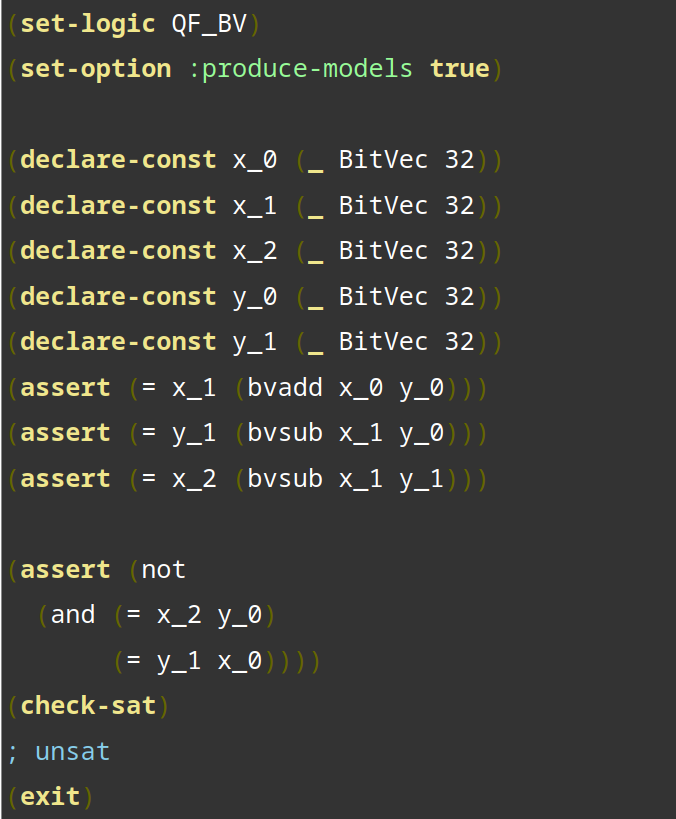
\includegraphics[width=\textwidth]{figures/l14/smt-example-bv.png}
	\end{minipage}
\end{frame}

\begin{frame}{SMT: Concluding Remarks}
	\textbf{SMT is a vast area -- we barely scratched the surface.}\\[4mm]
	
	\begin{minipage}{0.5\textwidth}
		\begin{itemize}
			\item Standardization of \highl{different theories \& logics}\\
			and their interactions
			\item SMT solvers support \highl{subsets of theories}
			\begin{itemize}
				\item Completely different reasoning needed\\
				for different theories, applications
			\end{itemize}
			\item Increasingly relevant research topic:\\
			\highl{Proofs for SMT solvers}
			\item Definitive resource surrounding SMT:\\
			\url{http://smt-lib.org/}
		\end{itemize}	
	\end{minipage}%
	\begin{minipage}{0.5\textwidth}
		\centering
		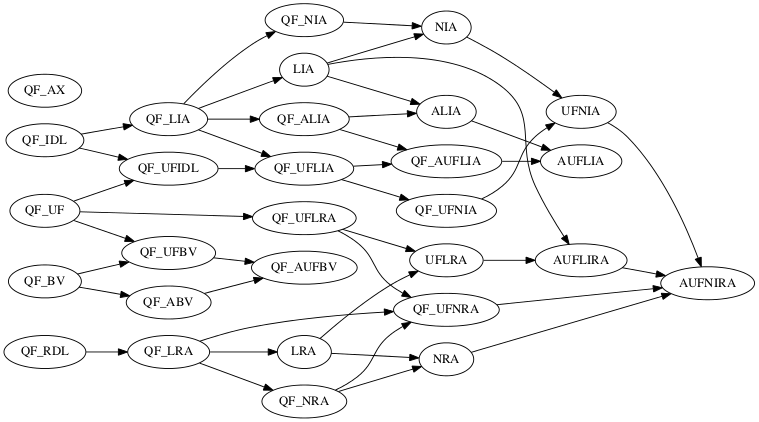
\includegraphics[width=\textwidth]{figures/l14/smtlib-logics.png}
	\end{minipage}
\end{frame}

\begin{frame}{References}
	\renewcommand*{\bibfont}{\scriptsize}
	\setlength\bibitemsep{3pt}
	\vspace*{-3mm}
	\printbibliography
\end{frame}

\end{document}
